% chktex-file 13

\documentclass{article}
\usepackage{amsmath}
\usepackage{amssymb}
\usepackage{hyperref}
\usepackage{xcolor}
\usepackage{ulem}
\usepackage{graphicx}
\usepackage[margin=0.5in]{geometry}
\usepackage[T1]{fontenc}

\graphicspath{ {./images/} }

\hypersetup{breaklinks=true}

\definecolor{darkblue}{rgb}{0, 0, 20}

\hypersetup{
    colorlinks=true,
    urlcolor=darkblue,
    linkcolor=blue,
    filecolor=magenta,
    citecolor=blue,
}

\setlength{\parindent}{0pt}

\begin{document}

\section*{Linear Recurrent Networks}

A Linear Recurrent Network is a type of recurrent model where the hidden state updates follow a purely linear recurrence.
\[h_t = Wh_{t-1}+Ux_t\]

Standard RNNs require sequential processing due to the non-linearity of their hidden states and the dependency on the previous one. By eliminating non-linearity, LRNs allow parallel computation using scan-based methods or matrix exponentiation, reducing time complexity from $O(N)$ to $O(\log N)$.

\section*{State Space Models}

A State Space Model models sequential data as a system of hidden states that change over time. An SSM models an input sequence $x(t)$ and maps it to an output $y(t)$ using a hidden state $h(t)$.
\[h'(t)=\mathbf{A}h(t)+\mathbf{B}x(t)\quad y(t)=\mathbf{C}h(t)\]
where $A$, $B$, and $C$, are system matrices that define how the state changes.
\vspace{1em}

To be used in deep learning models, the continuous equations are discretized at specific time steps. This enables parallel computation of all hidden states using scan-based methods or matrix exponentiation, making them highly scalable.
\[h_t=\mathbf{\overline{A}} h_{t-1} + \mathbf{\overline{B}} x_t\quad y_t = \mathbf{C}h_t\]
where the zero-order hold (ZOH) defines
\[\mathbf{\overline{A}}=e^{\Delta \mathbf{A}}\quad \mathbf{\overline{B}}={(\Delta \mathbf{A})}^{-1} (e^{\Delta \mathbf{A}} - \mathbf{I})\cdot \Delta\mathbf{B}\]
where $\mathbf{A}$ and $\mathbf{B}$ are fixed system matrices and $\Delta$ is a fixed step size.

\section*{Mamba (S6)}

While SSMs allow efficient sequence modeling with linear time complexity, they have limitations in their adaptability to the input. In a standard SSM, the hidden state updates are determined by the fixed system matrices. Mamba allows the hidden state parameters to be input-dependent and time-variant.
\[B = s_B (x)\quad C = s_C (x)\quad \Delta = \tau_\Delta (\text{Parameter} + s_\Delta (x))\]
where $s_B(x)=\text{Linear}_N(x)$, $s_C(x)=\text{Linear}_N(x)$, $s_\Delta(x)=\text{Broadcast}_D (\text{Linear}_1 (x))$, and $\tau_\Delta(x) = \text{softplus}(x)$. Broadcasting expands the dimension of the vector by copying the value $D$ times. Softplus, $\log(1+e^x)$, is a smooth approximation of the ReLU function.
\vspace{1em}

Also, SSMs do not guarantee long-term memory so Mamba uses High-Order Polynomial Projection Operators (HiPPO) to initialize $A$ in a way that retains long-term dependencies.

\section*{VMamba (SS2D)}

Instead of performing a one-dimensional scan on the data like S6, the 2D Selective Scan (SS2D) performs multi-directional scanning across a 2D grid for vision tasks. The image is flattened into four directional sequences, each corresponding to a different scan direction (left-right, right-left, top-bottom, bottom-top). Each sequence is processed independently with S6 blocks. The images are reconstructed from the outputs to form the four feature maps. The feature maps are summed through a Cross-Merge operation to form the final feature map.

\begin{center}
    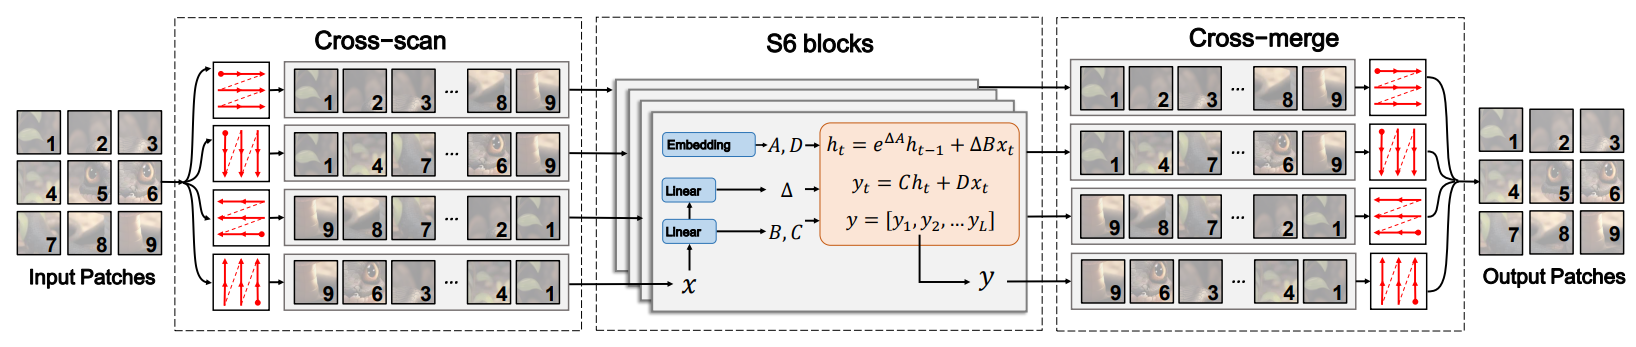
\includegraphics[scale=0.3]{vmamba-1.png}
\end{center}

\section*{Hamba}

The image is first passed through a Vision Transformer (ViT) to extract tokens, which are then downsampled with convolution layers. The Joints Regressor (JR) consists of stacked SS2D blocks and an MLP head to regress the initial MANO parameters. The Token Sampler (TS) uses the 2D joint locations from the JR to filter the initial tokens for relevance.
\vspace{1em}

The remaining tokens are passed through a Graph Convolution Network (GCN) and then concatenated with the global token mean to capture local and global joint relationships and build the Graph-guided State Space (GSS) tokens. The SS2D block is applied to the resulting tokens, rather than the image like in VMamba, and the SS2D output is concatenated to the GSS tokens. The GSS tokens are passed through a Layer Norm (LN) and Feed-Forward Network (FFN) and the output is concatenated to the GSS tokens.

\begin{center}
    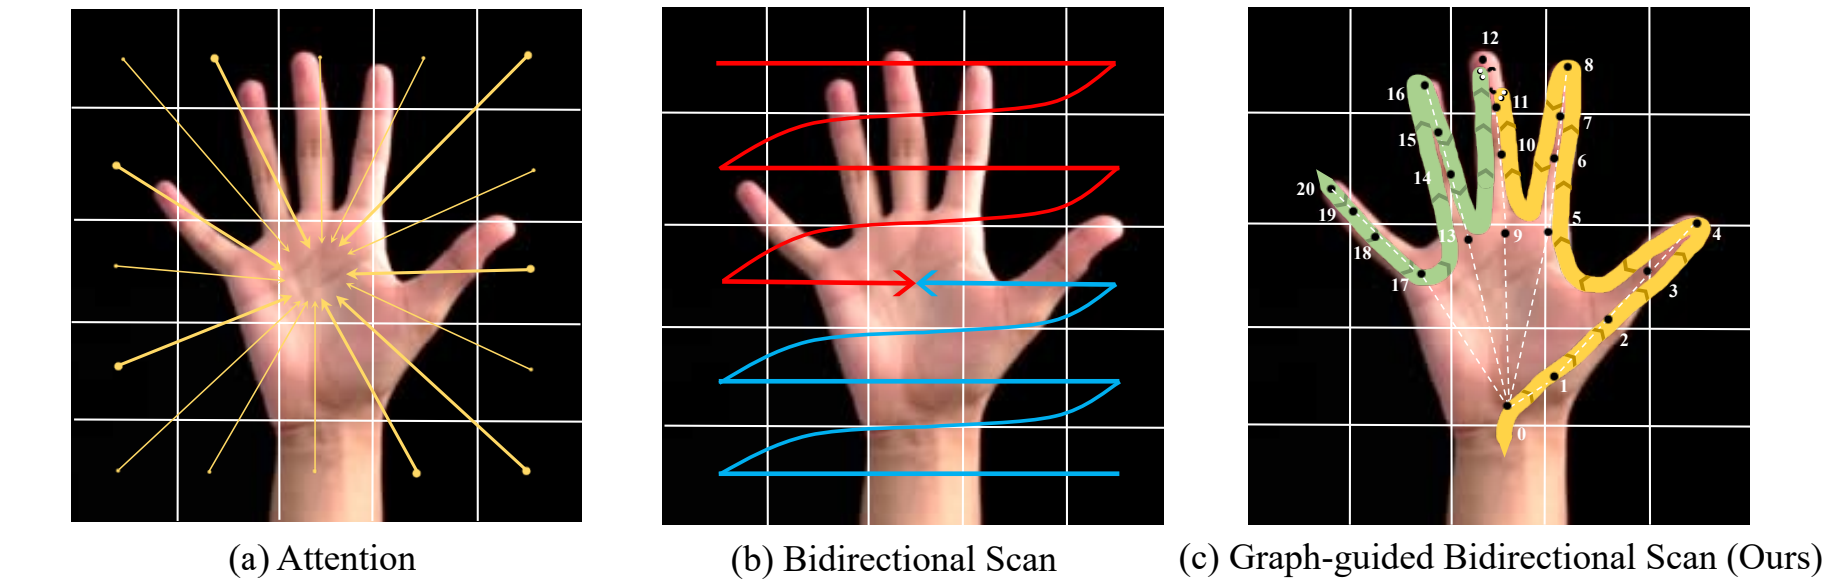
\includegraphics[scale=0.25]{hamba-3.png}
\end{center}

The global token mean, 2D joint locations, TS tokens, and GSS tokens, are concatenated and passed through a Multi-layer Perceptron (MLP) to regress the final MANO parameters.

\begin{center}
    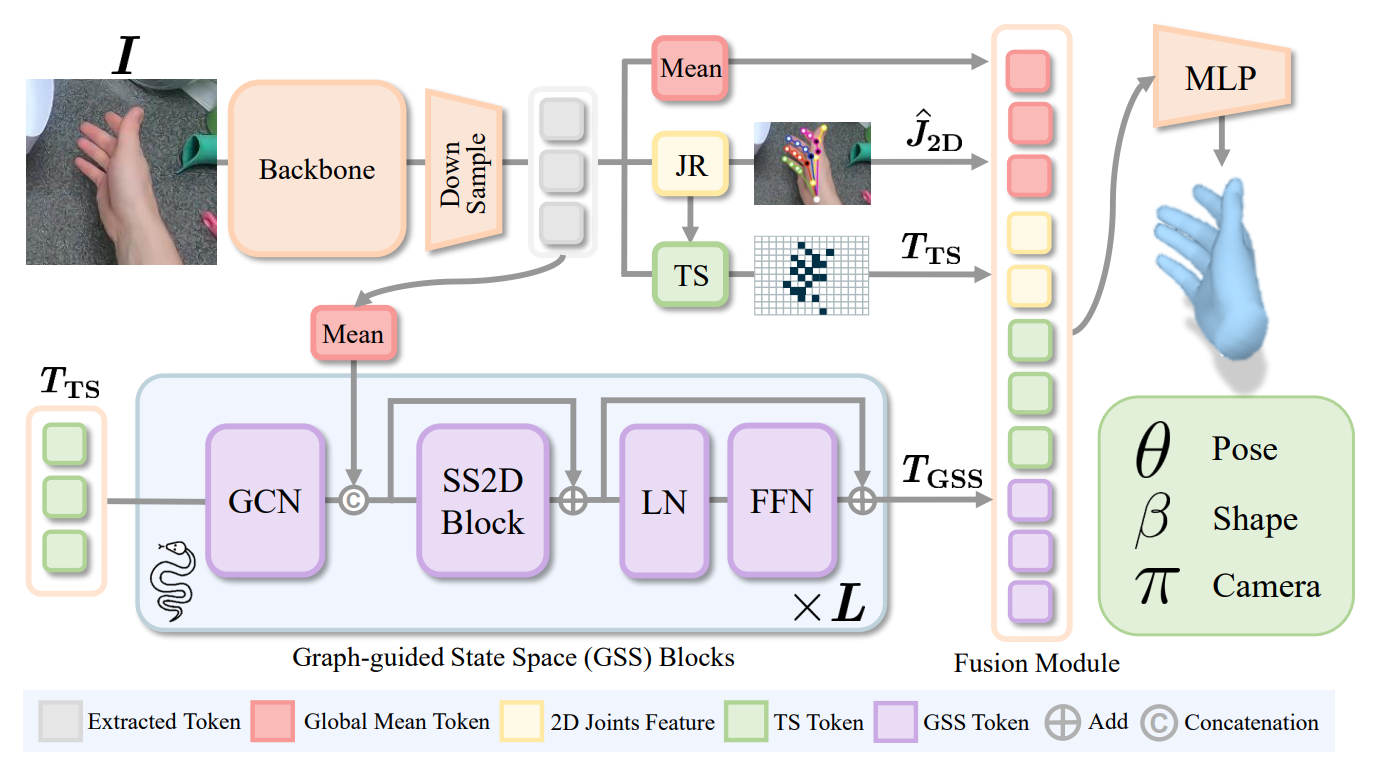
\includegraphics[scale=0.35]{hamba-1.png}
\end{center}

\pagebreak

\section*{Future Work}
\begin{enumerate}
    \item \textbf{Depth Estimation}
    
    Pass the image through a depth estimation network to generate a 2D depth map of the image. The depth map is concatenated with the image before passing it to the ViT backbone.

    \item \textbf{Object Pose Estimation}
    
    Instead of the 6D object pose keypoints, the ground truth labels are re-annotated to contain 8 3D keypoints that are predefined to best represent the surface for each object class.
    \vspace{1em}

    Two separate Hamba networks will be trained for hand and object reconstruction.
\end{enumerate}
\end{document}